\hypertarget{group__APACHE__CORE__CHARSET}{}\section{Charset Conversion}
\label{group__APACHE__CORE__CHARSET}\index{Charset Conversion@{Charset Conversion}}
Collaboration diagram for Charset Conversion\+:
\nopagebreak
\begin{figure}[H]
\begin{center}
\leavevmode
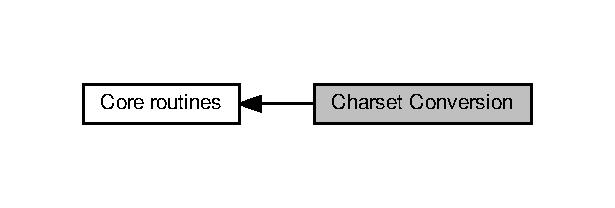
\includegraphics[width=295pt]{group__APACHE__CORE__CHARSET}
\end{center}
\end{figure}
These are the translation handles used to translate between the network format of protocol headers and the local machine format.

For an E\+B\+C\+D\+IC machine, these are valid handles which are set up at initialization to translate between I\+S\+O-\/8859-\/1 and the code page of the source code.~\newline
For an A\+S\+C\+II machine, they are undefined.

\begin{DoxySeeAlso}{See also}
ap\+\_\+init\+\_\+ebcdic() 
\end{DoxySeeAlso}
